\acresetall
\chapter{Design and Implementation}\label{ch:chapter3}

In this chapter we will discuss the design, including the threat model and assumptions made, and the implementation choices that we made for this research.	

\section{Overview}\label{sec:overview}

\par In this research, we leverage the Xen’s \ac{VMI} capabilities to create a mechanism that protects some critical files on a \ac{VM}'s mounted filesystem by monitoring the systems calls that are being invoked. We will create an additional \ac{ACL} on the hypervisor that will include modified permissions for file access. The above permissions are different compared to those on the guest \ac{VM}, allowing for the enforcement of different file access policy than the ones enforced by the guest \ac{VM}. The hypervisor will externally monitor which files are being accessed and cross-check the requested permissions with its \ac{ACL}, which we call \ac{SACL}, entries providing this way additional safety for high-value files, even while under \ac{VM} compromised attacks. Although a similar approach was employed with Paladin~\cite{baliga2008automated} and Nasab~\cite{nasab2012security}, there are some fundamental differences. 

\par Before continuing we need to establish why our solution is secure. We chose to monitor which files are being accessed by trapping on the system calls that are being invoked. This choice covers all cases for opening a file on a mounted filesystem. The reason is the way the Linux \ac{OS} is designed. To provide higher security most \acp{OS}, including Linux, operate in two modes. One is called \emph{User Mode}, a non-privileged mode of operation used by normal applications, and \emph{Kernel Mode}, a privileged mode of operation used from the \ac{OS}, as mentioned in ~\cite{linuxkernel} and explained in more detail later in this chapter. Because the kernel is a very complex software, and to ensure secure execution of code, linux employs specific entry points to the kernel code, which is an \ac{API} for applications to interact with the kernel. This \ac{API} is called system calls. 

\par As mentioned in \cite{linuxkernel}, a User Mode process cannot access directly the hardware. Each file operation must be performed in Kernel Mode. The \ac{OS} will not allow direct access to hardware. If a process needs file access, it needs to perform a system call, asking this way the \ac{OS} for the desired operation. The \ac{OS} checks if the request is valid and if it is the \ac{OS} accesses the file on behalf of the process and returns to the process the result of the operations, as shown in \ref{fig:syscall}. This requirement, to make a system call for all file operations, provides the place in the \ac{OS} executable code, which if we monitor we can extract the information of all files being accessed. So, we cannot miss any file any process will try to open.

\begin{figure}[ht]
	\centering
	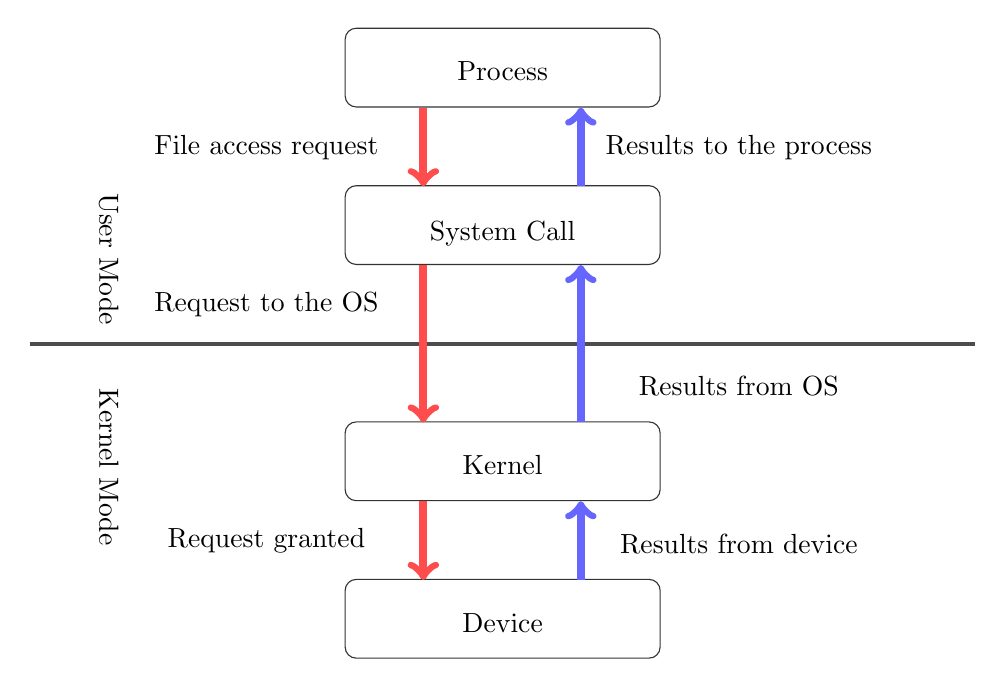
\begin{tikzpicture}[
rednode/.style={circle, draw=red!60, fill=red!30, very thick, minimum size=5mm, text width=2cm, text centered},
bluenode/.style={rectangle, draw=black!60, fill=blue!20, very thick, minimum size=5mm, text width=2cm, text centered},]



\node (rect) [anchor= south west, fill=white, rectangle, draw=black!80, rounded corners, minimum width=40mm, minimum height=10mm, label={[yshift=-0.8cm]Process}] at (2, 0) {}; 

\node (rect) [anchor= south west, rectangle, rounded corners, minimum width=20mm, minimum height=10mm, label={[yshift=-0.9cm]File access request}] at (0, -0.9) {}; 

\node (rect) [anchor= south west, rectangle, rounded corners, minimum width=20mm, minimum height=10mm, label={[yshift=-0.9cm]Results to the process}] at (6, -0.9) {}; 

\node (rect) [anchor= south west, fill=white, rectangle, draw=black!80, rounded corners, minimum width=40mm, minimum height=10mm, label={[yshift=-0.9cm]System Call}] at (2, -2) {}; 

\node (rect) [anchor= south west, rectangle, rounded corners, minimum width=20mm, minimum height=10mm, label={[yshift=-0.9cm]Request to the \ac{OS}}] at (0, -2.9) {}; 

\node (rect) [anchor= south west, rectangle, rounded corners, minimum width=20mm, minimum height=10mm, label={[yshift=-0.9cm]\rotatebox{270}{User Mode}}] at (-2, -3) {}; 

\draw[anchor= south west, draw=black!70, line width=0.5mm,-] (-2, -3) -- (10, -3);

\node (rect) [anchor= south west, rectangle, rounded corners, minimum width=20mm, minimum height=10mm, label={[yshift=-0.7cm]\rotatebox{270}{Kernel Mode}}] at (-2, -6) {}; 

\node (rect) [anchor= south west, fill=white, rectangle, draw=black!80, rounded corners, minimum width=40mm, minimum height=10mm, label={[yshift=-0.8cm]Kernel}] at (2, -5) {}; 

\node (rect) [anchor= south west, rectangle, rounded corners, minimum width=20mm, minimum height=10mm, label={[yshift=-0.9cm]Results from \ac{OS}}] at (6, -3.9) {}; 

\node (rect) [anchor= south west, rectangle, rounded corners, minimum width=20mm, minimum height=10mm, label={[yshift=-0.9cm]Request granted}] at (0, -5.9) {}; 

\node (rect) [anchor= south west, rectangle, rounded corners, minimum width=20mm, minimum height=10mm, label={[yshift=-0.9cm]Results from device}] at (6, -5.9) {}; 

\node (rect) [anchor= south west, fill=white, rectangle, draw=black!80, rounded corners, minimum width=40mm, minimum height=10mm, label={[yshift=-0.8cm]Device}] at (2, -7) {}; 

\draw[anchor= south west, draw=red!70, line width=1mm,->] (3, 0) -- (3, -1);
\draw[anchor= south west, draw=red!70, line width=1mm,->] (3, -2) -- (3, -4);
\draw[anchor= south west, draw=red!70, line width=1mm,->] (3, -5) -- (3, -6);

\draw[anchor= south west, draw=blue!60, line width=1mm,<-] (5, 0) -- (5, -1);
\draw[anchor= south west, draw=blue!60, line width=1mm,<-] (5, -2) -- (5, -4);
\draw[anchor= south west, draw=blue!60, line width=1mm,<-] (5, -5) -- (5, -6);


%\draw[anchor= south west, draw=red!70, line width=1mm,->] (4.5, 2) -- (7.2, 2);
%\draw[anchor= south west, draw=red!70, line width=1mm,->] (9.2, 2) -- (9.6, 2);
%\draw[anchor= south west, draw=red!70, line width=1mm,->] (11.6, 2) -- (12.2, 2);

%\draw[anchor= south west, draw=blue!60, line width=1mm,->] (12.2, 1) -- (1, 1) -- (1, 3.5);
%\draw[anchor= south west, draw=blue!60, line width=1mm,->] (1, 4.5) -- (1, 5);



\end{tikzpicture}
	\caption{System call information flow}
	\label{fig:syscall}
\end{figure}

\par Table 12.1 in \cite{linuxkernel} shows the list of system calls relevant to filesystems. According to that table, the system calls of importance to us are \emph{open(), rename(), unlink()} and \emph{truncate()}. Some of these system calls have been evolved over time to provide better security and to eliminate problems. Such an evolved system call is \emph{openat()}. Going through the available system call list in \emph{/usr/include/asm/unistd\_64.h}, we assess that the system calls mentioned in table~\ref{tbl:syscalls}, where number is the system call number as it is passed to the kernel, provide full coverage of the possible ways a file can be accessed when being on a mounted device. 

\begin{table}[ht]
	\centering
	\caption{Trapped system calls}
	\label{tbl:syscalls}
	\begin{tabular}{cc}
		\toprule
		System call & Number \\
		\hline
		open & 2 \\ 
		openat & 257 \\ 
		name\_to\_handle\_at & 303 \\
		open\_by\_handle\_at & 304 \\
		rename & 82 \\ 
		renameat & 264 \\  
		renameat2 & 316 \\ 
		unlink & 87 \\ 
		unlinkat & 263 \\
		truncate & 76 \\
		\bottomrule
	\end{tabular}	
\end{table}



\section{Threat Model}\label{sec:threat}

Computer security has been evolving because the attackers methods evolve, too. Modern \acp{OS} and applications are so complex that they introduce many bugs in their code. Some of these bugs are benign, but some are serious enough to allow security breaches like remote access to a system, administrator/root access, arbitrary code execution, etc..

\par For this research, we have adopted a moderate threat model where we assume that the guest \ac{VM} is insecure. That means that an adversary can gain access to it remotely. We also assume that physical access to the hosting machine is restricted and the attacker cannot use physical media like USB sticks or CD-ROMs to compromise the host system. This reflects many applications and systems working over a network connection as well as cloud solutions. The files we want to protect are on a mounted disk.

\par Moreover, we assume that the \ac{OS} installed on the guest \ac{VM} is not trusted. This essentially means that the adversaries can gain root privileges, allowing them this way to modify system executables, as well as load kernel modules during runtime. This allows for kernel memory modification. Although an adversary can manipulate some of the memory values before a system call gets executed, such as the file being accessed, most of them will not affect the outcome. There are two values in a process's memory space though, which if modified can alter the overall behavior. These values are the \emph{userid} and \emph{groupid} of the process. \emph{--I don't know if I will have the time to complete this protection. We could leave it as future work. I have an idea on how to do it, I just don't think I can finish all by September.--}

\par We consider the hypervisor along with its Dom0 to be secure and trusted. We will not address hypervisor vectored attacks.

\par When launching a \ac{VM} there might be a small time window when the guest \ac{VM} is running without the protection of our system. Until we find a way to find the exact time LibVMI can be initialized to protect the guest \ac{VM}, we will consider attacks that modify the running system during boot-time outside the scope of this research.

\section{Requirements}\label{sec:requirements}
The goal of this research is to provide a virtualization extension that will extend the granular-level file access control of the Linux \ac{OS}. The requirements we defined for our system are:
\begin{itemize}
	\item \textbf{(R1)} The solution must be Out-VM, to avoid modification from the potential adversary. 
	\item \textbf{(R2)} The system must remain efficient and usable, by not introducing significant overhead on the runtime of the \ac{VM}, as well as by not enforcing many restrictions to the users. 
	\item \textbf{(R3)} The coverage of the relevant system calls must be maximum.
\end{itemize}


\section{Design}\label{sec:design}

\par We will use a type-I hypervisor instead of type-II, as type-I hypervisors are more efficient and deployed more as a commercial solution, while type-II are used mostly for testing and analysis. We chose the Xen hypervisor as it is open source and is used widely, so the results of the research can be used in a variety of applications. By leveraging Xen's introspection methods, we will create the Out-VM monitoring agent, which will run on Dom0, completely outside the \ac{VM}, conforming this way with \textbf{(R1)}. Also, by ensuring that there is no code running on the guest \ac{OS}, we increase the deployment speed, as there is no need to modify the guest \ac{VM} in any way. The required pre-deployment configuration for the guest \ac{VM} is kept to a minimum and does not involve any modification, only information gathering.

\par As a platform to base our solution, we chose DRAKVUF~\cite{lengyel2014drakvuf}. DRAKVUF will provide us a stealthy monitoring base, as it leverages alternate \ac{EPT}s with different permissions, preventing any detection from applications inside a \ac{VM}. We will have to restrict some of the usability of the system, although not during normal execution, to achieve the file confidentiality, integrity and availability we want, as explained later in this chapter. Therefore we assume that \textbf{(R2)} is achieved in the part of restrictions, although a few restrictions apply, mostly concerning the root user. Overhead and usability of the system will be discussed in chapter \ref{ch:chapter4}.

\par We will employ the stealthy property of DRAKVUF to make the process of file protection completely transparent to the guest \ac{OS}, retaining a zero-footprint monitor on the guest. DRAKVUF also helps bridge the semantic gap between the hypervisor and the \ac{VM} with the use of a Rekall profile~\cite{rekall}, having access to selected kernel structures. Furthermore, we want to employ a per user \ac{ACL}, enforced on specific files or whole folders, which are sometimes not essential to the \ac{OS}, but essential to the user. Generally, we want to protect any type of data, regardless of the content. We improve confidentiality by denying even read access, integrity by denying write, and availability by protecting deletion or moving of the files. This mechanism must also extend to the root user, since our threat model assumes that the system is compromised. To achieve that, we will intercept all relevant system calls from all users and verify the validity of the request. 

\par Monitoring the execution of the system calls in table \ref{tbl:syscalls} and validating the request made to the guest \ac{OS} kernel is sufficient for ensuring the guest \ac{VM} file confidentiality, integrity and availability, as we want to enforce it, thus conforming to \textbf{(R3)}.


\section{Implementation}\label{sec:implementation}

\par Following we expand on how we implemented the mechanism to provide the file access security of our system.



\subsection{Shadow Access Control List}\label{sub:sacl}
During the initialization of our DRAKVUF plugin, we read the \ac{SACL}s we have created for the \ac{VM} to be protected. At this point of the research we were limited to small lists, so the initial implementation for storing and searching through the \ac{SACL}s is two linked lists and two arrays of linked lists, as explained below. Figure~\ref{fig:sacl_layout} depicts the structure created for storing each entry.

\begin{figure}[ht]
	\centering
	\begin{tabular}{|c|c|}
		\hline
		\textbf{Variable Name} & \textbf{Variable type} \\
		\hline
		pathname & char * \\
		\hline
		mode & unsigned int \\
		\hline
		u & uid\_t \\
		\hline
		g & gid\_t \\
		\hline
		next & struct protected\_files * \\
		\hline
	\end{tabular}
	\caption{\textit{struct protected\_files} memory layout}
	\label{fig:sacl_layout}
\end{figure}

\par The above memory structure is used for both protected folders and protected files. Moreover, we create two of each, as mentioned before, one for the root user and one for the rest. To improve overall search speed for our algorithm, instead of keeping one linked list for all the files, we created two arrays, one for the root user and one for the rest, of size 4096 for the files, which is the maximum pathname length, as set in \textit{linux/limits.h}. Then, according to the pathname length of each entry, it is appended to a linked list located at the array in index equal to the pathname length. 

\par In the \ac{SACL} files the permissions are set according to the Linux permission bits schema. This means that the last 3 digits of the \textit{mode} field, when encoded in octal form, define the permissions we want to enforce. The first one defines the owner rights, the second the group rights, and the third the other user rights. The number itself is the sum of the permissions 4 for read, 2 for write, and 1 for execute. As an example, if we encounter or set permissions 744, it means that the owner can read, write and execute the file, while anyone in the same group and everyone else can only read the file.

\par The \ac{SACL}'s format was kept as simple as possible so that editing and reviewing it is easy. Additionally, by keeping the format of the Linux \ac{ACL}, we provide to the system administrator a familiar permissions schema, so it is easier to understand and manage. Figure~\ref{fig:sacl} shows an example, which we will analyze later.

\begin{figure}[ht]
	\centering
	\begin{lstlisting}
/home/user/Documents/readme.txt		100644	1000	1000
/home/user/Desktop/credit_card.pdf	100400	1000	1000
/home/user/Documents			140220	0	0
	\end{lstlisting}
	\caption{\ac{SACL} sample}
	\label{fig:sacl}
\end{figure}

\par The system keeps two \acp{SACL}: one for all non-root users and one for root, since this account is of greater significance. Furthermore, two different checks are being performed. First it checks for a protected folder, as it is a more generic case. If no entry is found, it then checks for specific files in the list to match. 

\par We chose to create two separate \acp{SACL} to reduce the performance overhead of our solution. By making this separation we allow for the program to automatically eliminate entries in the \ac{SACL} that need not be checked against. If a program or service runs as root, we do not need to check the entries that apply to the rest of the users and vice versa. Additionally, since the root user account will always run on a system, because the \ac{OS} runs under this account, root will constantly open files relevant to the running of the \ac{OS}. Therefore, we assess that adding more entries to match against in the \ac{SACL} will introduce a performance overhead we can avoid with the separation we implemented. Besides this coarse refinement of the \ac{SACL} entries, the level of protection applied to the files is the same, whether applied to the root user or any other user.

\par As we see in figure~\ref{fig:root_sacl}, the \ac{SACL} for protecting files from the root user is more simple. Since it is targeted for this specific user, we do not need the entries for owner and group. Furthermore, the permission bits for group and others are ignored when parsed. This simplifies the file structure, while at the same time reduces memory utilization.

\begin{figure}[ht]
	\centering
	\begin{lstlisting}
	/etc/shadow     100400
	/etc/pam.d/su   100000
	\end{lstlisting}
	\caption{root user \ac{SACL} sample}
	\label{fig:root_sacl}
\end{figure}


\par Before moving on, we must emphasize that the system does not alter basic properties of the files that are being protected. It does not change the owner or the group, since this requires intervention in the \ac{VM}. Although in the \ac{SACL} we can define a different owner, the generic effects is denial of access. That means that we cannot change who can access a file, rather we can change who cannot. This system acts as a supplementary and more fine-grained access control mechanism to make more strict file access policies. Therefore, if we change the owner of a file in the \ac{SACL}, we essentially prohibit access to that file by the owner; we do not specify a new one, as the final call for file access comes from the unmodified guest \ac{OS}.



\subsection{System Calls}\label{sub:syscalls}


\par All applications running in user-space need to ask the kernel to access a file. Applications do not have knowledge of the low-level \ac{OS} and device details to access the files they need, so they request from the kernel to do that work for them. The kernel accesses the requested file using the device drivers and, when the operation is completed, returns to the application a handle to that file, called file descriptor. This happens for many operations restricted to the kernel for security reasons. Also, it provides an abstraction to the applications, which are written without the need of the knowledge of device specifics and work on variations of the underlying hardware running the same \ac{OS}. 

\par For applications to be compatible to \ac{OS} version upgrades and portable between different systems, a specific standard calling convention of these kernel functions is needed. This calling convention is a system call. System calls are specific entry points to the kernel, which, when provided specific arguments perform an operation on behalf of the application. Many system calls exist, each performing a different operation. We will focus on those who are relevant to accessing files, whether to read or modify. These are depicted in table~\ref{tbl:syscalls}.

\par To gain the insight on what files are being accessed, we need to know whenever this event happens. We will use DRAKVUF to create a trap on all the afore-mentioned system calls.

\par This gives us the opportunity to stop the \ac{VM} execution when these system calls are called. At this point, we access the registers related with each system call to retrieve the information we need to perform the validation of the requested call. Figure~\ref{fig:overview} gives an overview of the flow of information during a trapped system call. 

\par The arguments to the system calls for the 64-bit Linux \ac{OS} we used as our test platform are passed to the kernel through the registers in the order of rdi, rsi, rdx, r10, r8, r9, while the system call number is passed in rax. Table~\ref{tbl:prototypes} shows which arguments need to be passed to each system call on each register for it to perform the requested operation.

\begin{table}[ht]
	\centering
	\footnotesize
	\caption{Trapped system calls}
	\label{tbl:prototypes}
	\begin{tabular}{ccccccc}
		\toprule
		Syscall 				&           	&  				& 						&  						&  					&   		\\
		Name 					& rax		  	& rdi 			& rsi 					& rdx 					& r10 				& r8 		\\
		\toprule
		open 					& 2 			&	const char	&	int flags			&	int mode			&					&		 	\\
								&   			&	*pathname	&						&						&					&		 	\\
		\hline
		openat	 				& 257  			&	int dirfd	&	const char 			&	int flags			&	int mode		&	 		\\
								&   			&				&	*pathname			&						&					&		 	\\
		\hline
		name\_to\_handle\_at 	& 303  			&	int dirfd	&	const char			&	struct file\_handle	&	int				&	int	 	\\
								&   			&				&	*pathname			&	*handle				&	mount\_id		&	flags 	\\
		\hline
		open\_by\_handle\_at 	& 304  			&	int mountfd	&	struct file\_handle	&	int	flags			&					&		 	\\
								&   			&				&	*handle				&						&					&		 	\\
		\hline
		rename 					& 82  			&	const char	&	const char			&						&	 				&		 	\\
								&   			&	*oldpath	&	*newpath			&						&					&			\\
		\hline
		renameat 				& 264  			&	int 		&	const char 			&	int 				&	const char 		&	 		\\
								&   			&	olddirfd	&	*oldpath			&	newdirfd			&	*newpath		& 			\\ 
		\hline
		renameat2 				& 316  			&	int			&	const char 			&	int 				&	const char 		&	unsigned\\
								&   			&	olddirfd	&	*oldpath			&	newdirfd			&	*newpath		& 	int flags\\ 
		\hline
		unlink 					& 87  			&	const char	&						&						&					&		 	\\
								&   			&	*pathname	&						&						&					&		 	\\ 
		\hline
		unlinkat 				& 263  			&	int dirfd	&	const char			&	int flag			&					&		 	\\
								&   			&				&	*pathname			&						&					&		 	\\
		\hline
		truncate 				& 76  			&	const char	&	off\_t				&	int flag			&					&		 	\\
								&   			&		*path	&	length				&						&					&		 	\\
		\bottomrule
	\end{tabular}	
\end{table}

\subsection{System Call Hooking}\label{sub:hooking}

To achieve the above mentioned system call intercept we need to place traps to the system calls of interest. This gets implemented by DRAKVUF. LibVMI reads the Rekall profile of the guest \ac{VM} to get the base address of the kernel symbol table. DRAKVUF then starts from that base address and searches for the system call table. This table includes the function pointers for all supported system calls. Going through that table makes possible the detection and trapping of the system calls. This is achieved by placing the \textit{INT3 (0xCC)} byte at the beginning of the system call function. This byte is executed by the \ac{CPU} as a debugging interrupt, a breakpoint. This in its turn triggers a VM-exit, which is caught by DRAKVUF and handled by our callback function. DRAKVUF implements multiple \ac{EPT}s with different permissions for the same page. This allows placing the trap in the system calls, while at the same time when accessed for read, the original functions are accessed, not revealing this way the injected breakpoint.

\par Table~\ref{tbl:prototypes} shows that there are two generic cases we need to examine. One case is for the \emph{open()}, \emph{rename()} and \emph{unlink()} system calls, where we have to find the strings pointer by the pointers in the \emph{rdi} register, and in the \emph{rsi} register in the case of \emph{rename()}. After we retrieve the strings, we then try to match them to any entry in the \ac{SACL}s in the hypervisor. If there is a match, we then retrieve the \emph{userid} and \emph{groupid} of the owner of the currently running process, which requested the specific file access. We check then if the user or group of the running process has enough permissions to access the files, according to the \ac{SACL}s. If there is any difference between the permissions and the requested access mode, we overwrite the contents of the relevant registers with NULL, resulting in a failed system call.

\par The second case is for the \emph{openat()}, \emph{renameat()} and \emph{unlinkat()} system calls, where we have to retrieve the string of the file being accessed from different registers, according to table~\ref{tbl:prototypes}. After that the algorithm is the same as above.


\begin{figure}[ht]
	\centering
	\begin{tikzpicture}[
rednode/.style={circle, draw=red!60, fill=red!30, very thick, minimum size=5mm, text width=2cm, text centered},
bluenode/.style={rectangle, draw=black!60, fill=blue!20, very thick, minimum size=5mm, text width=2cm, text centered},]

  
   	\node[anchor= south west, copy shadow={draw=black!10, fill=black!40, opacity=0.5}, fill=white, rectangle, rounded corners, draw=black, minimum width=50mm, minimum height=80mm, label={[yshift=-1cm]north:Dom0}] at (0, 0) {};
   	
	\node[dashed, anchor= south west, fill=white, rectangle, draw=black!80, rounded corners, minimum width=45mm, minimum height=10mm, label={[yshift=-0.8cm]\ac{SACL}}] at (0.25, 6) {}; 
	\node[anchor= south west, fill=white, rectangle, draw=black!80, rounded corners, minimum width=45mm, minimum height=10mm, label={[yshift=-0.9cm]DRAKVUF Plugin}] at (0.25, 4.5) {}; 
	\node (rect) [anchor= south west, fill=white, rectangle, draw=black!80, rounded corners, minimum width=45mm, minimum height=10mm, label={[yshift=-0.8cm]LibVMI}] at (0.25, 3) {}; 
	
%	\node[dashed, anchor= south west, fill=white, rectangle, draw=black!80, minimum width=20mm, minimum height=15mm, label={[yshift=-1.5cm]\begin{tabular}{c}
%		System \\ Map
%		\end{tabular}}] at (2.5, 1.5) {}; 
	
	
   	\node[anchor= south west, copy shadow={draw=black!10, fill=black!40, opacity=0.5}, fill=white, rectangle, rounded corners, draw=black, minimum width=50mm, minimum height=70mm, label={[yshift=-0.7cm]north:User VM (DomU)}] at (7, 0) {};
	
	\node[anchor= south west, fill=white, rectangle, draw=black!80, rounded corners, minimum width=45mm, minimum height=10mm, label={[yshift=-0.8cm]User-level Application}] at (7.25, 4.5) {}; 
	\node[anchor= south west, fill=white, rectangle, draw=black!80, rounded corners, minimum width=45mm, minimum height=10mm, label={[yshift=-0.8cm]System Call}] at (7.25, 3) {}; 
	
	

%	\node[dashed, anchor= south west, fill=white, rectangle, draw=black!80, minimum width=20mm, minimum height=20mm, label={[yshift=-1.7cm]\begin{tabular}{c}
%		Page \\ Directory
%		\end{tabular}}] at (7.2, 1.5) {}; 
%
%	\node[dashed, anchor= south west, fill=white, rectangle, draw=black!80, minimum width=20mm, minimum height=20mm, label={[yshift=-1.7cm]\begin{tabular}{c}
%	Page \\ Table
%	\end{tabular}}] at (9.6, 1.5) {}; 
%
%	\node[dashed, anchor= south west, fill=white, rectangle, draw=black!80, minimum width=20mm, minimum height=20mm, label={[yshift=-1.7cm]\begin{tabular}{c}
%	Kernel \\ Data
%	\end{tabular}}] at (12.2, 0.5) {}; 
%
	\draw[anchor= south west, draw=red!70, line width=1mm,->] (8, 4.5) -- (8, 4);
	\draw[anchor= south west, draw=red!70, line width=1mm,->] (8, 3) -- (8, 2.5) -- (4, 2.5) -- (4, 3);
	\draw[anchor= south west, draw=red!70, line width=1mm,->] (4, 4) -- (4, 4.5);
	\draw[anchor= south west, draw=red!70, line width=1mm,->] (4, 5.5) -- (4, 6);
			
	\draw[anchor= south west, draw=blue!70, line width=1mm,<-] (11, 4.5) -- (11, 4);
	\draw[anchor= south west, draw=blue!70, line width=1mm,<-] (11, 3) -- (11, 1.5) -- (1, 1.5) -- (1, 3);
	\draw[anchor= south west, draw=blue!70, line width=1mm,<-] (1, 4) -- (1, 4.5);
	\draw[anchor= south west, draw=blue!70, line width=1mm,<-] (1, 5.5) -- (1, 6);



\end{tikzpicture}
	\caption{Information flow during a trapped system call execution}
	\label{fig:overview}
\end{figure}


\subsection{The task struct}\label{sub:struct}
A crucial part in the design of our solution is the Linux kernel \textit{task\_struct}. It a complex structure where the kernel stores many information concerning the running processes. Each running process is assigned one such structure by the kernel, so that the kernel can monitor the process and retrieve various information about it. A special macro, \textit{current}, points directly to the current running process. We need to map this structure and find the address offsets of the information we need. We will revisit the \textit{task\_struct} in the next sections, as we mention what we need to access.

\par Although normally this process is not complex, in our case there are some challenges. The first is that we need to find the correct offsets inside the \textit{task\_struct} for the entries we want, which depend on the kernel version. Furthermore, we need to make constant conversions between \ac{GMFN} and \ac{MFN}, as the memory values we retrieve correspond to the \ac{VM}s address space, but we need to access the actual physical memory to read the information we require.


\subsection{Trap Handling}\label{sub:handling}

After a hooked system call gets executed, our callback function is called. We firstly retrieve the file that is being accessed and by which process, by getting its process id (figure~\ref{fig:getfile}). 

\begin{figure}[ht]
	\centering
	\begin{lstlisting}[ basicstyle=\footnotesize]
currpid = vmi_dtb_to_pid(vmi, info->regs->cr3);
switch (info->regs->rax){
case S_OPEN:
case S_RENAME:
case S_UNLINK:
	addr=vmi_translate_uv2p(vmi,info->regs->rdi,currpid);
	filename=vmi_read_str_pa(vmi,addr);
	.
	.
	break;
case S_OPENAT:
case S_UNLINKAT:
case S_RENAMEAT:
case S_RENAMEAT2:
	addr=vmi_translate_uv2p(vmi,info->regs->rsi,currpid);
	filename=vmi_read_str_pa(vmi,addr);
	.
	.
	break; }
	\end{lstlisting}
	\caption{Getting the file being accessed}
	\label{fig:getfile}
\end{figure}


\par When a system call is executed the file being accessed is passed either with absolute, or relative path. The first case is straightforward, as by reading the string pointer by the corresponding register, we retrieve the full pathname of the file. If the file is passed with a relative path, the retrieval procedure is more complicated. That is because we need to recreate the \ac{PWD}. The Linux kernel does not store this information somewhere. On the contrary, in the \textit{task\_struct}, the kernel only stores in another structure the parent directory. Therefore, we need to loop through the parent folders, so that by prepending each time the parent, we recreate the \ac{PWD} and the full pathname. To achieve this we created a new function that walks though the \emph{task\_struct} to collect all the required information. This allows us to try to match the file being accessed with the entries in the \ac{SACL}.

\par After we have retrieved the pathname, we then check for the system call that triggered the VM-exit event. For this research we will not handle the \textit{name\_to\_handle\_at()} and \textit{open\_by\_handle\_at()} system calls. At this point of the research we are unaware of any compiled program that uses this specific system call. Moreover, although this is a valid and known attack vector to bypass this solution, support for it can be added in the future, while at the same time does not hinder our proof of concept. The rest of the system calls are handled as follows: 
\begin{itemize}
	\item \textit{open()} with \textit{openat()}
	\item \textit{rename()} with \textit{renameat()} and \textit{renameat2()}
	\item \textit{unlink()} with \textit{unlinkat()}
\end{itemize}

\par In the case of \textit{unlink()} and \textit{unlinkat()}, which are used for file deletion the procedure is straightforward. Once we look in the \ac{SACL}, if there is an entry, we verify that the user or group deleting the file, has write permissions. If that is true, the callback function returns control to the \ac{VM} to resume execution. If permissions do not match, the pointer to the filename string is modified to \textit{NULL}, so that the system call, after the \ac{VM} resumes execution, fails (figure~\ref{fig:unlink}). By hooking and preventing execution of these system calls we prevent deletion of the protected files, improving this way the availability assurances of the underlying \ac{OS}.

\begin{figure}[ht]
	\centering
	\begin{lstlisting}[ basicstyle=\footnotesize]
case S_UNLINK:          
case S_UNLINKAT:  switch(info->userid){
case ROOT: // root user
	if(strcmp(check->pathname,filename)==0){
		check_permissions(check,info,vmi,ROOT);			
	.
	.
	break;
default: // other users
	if (strcmp(check->pathname,filename)==0){
		if (check->u == info->userid){
			check_permissions(check,info,vmi,USER);}
		else if (check->g == info->groupid){
			check_permissions(check,info,vmi,GROUP);}
	else {
		check_permissions(check,info,vmi,OTHER);}}
	.
	.
	break;}
	\end{lstlisting}
	\caption{unlink() and unlinkat() skeleton code flow}
	\label{fig:unlink}
\end{figure}

\par The search for a match in the \ac{SACL}s is performed in two steps for all cases. Once to go through protected folders and once to go through individually protected files. Also, the root user is handled separately from the rest of the users because of the special elevated privileges that account is granted. 

\par In the case of \textit{rename()}, \textit{renameat()} and \textit{renameat2()}, which are used for file moving, we perform the same check as per \textit{unlink()} and \textit{unlinkat()}, with the difference that if we do not find a match for the \textit{oldname} of the system call, we additionally check for a match on the \textit{newname}. The first part ensures that if the user or group does not have read permissions, as enforced by our \ac{SACL}, he cannot rename or move the file to an unprotected folder or filename, ensuring the confidentiality of the information stored in the file. In the second case we prevent the protected file from being overwritten by another file, if the permissions are not correct. This way we improve integrity of the underlying \ac{OS}, by preventing modification of the protected file. 

\par Finally in the case of \textit{open()} and \textit{openat()}, we only have to check for one filename in our \ac{SACL}s. If there is an entry, then the permission check algorithm is more complicated. This happens because we have to match the requested by the process access \textit{mode} with the permissions we want to enforce. So, we check for read permission when a \textit{O\_RDONLY} access is requested, and for write permissions on a \textit{O\_WRONLY}. In the case of a \textit{O\_RDWR} request we initially check for both permissions. If that fails, we then check if the process user or group has read permissions. If that is true, we alter the file access mode to read-only and allow execution. If all of them fail we change the \textit{rax} register contents to \textit{NULL} and resume \ac{VM} execution, which results to a failed system call. This more complex permission check improves confidentiality, by not allowing read access to those who do not have the right, and integrity and availability by denying write access to those who cannot write to the file, as per the \ac{SACL} enforced policy. Figure~\ref{fig:open} shows the code for the permission checks done in case of the \textit{open} and \textit{openat} system calls.




\begin{figure}[ht!]
	\centering
	\begin{lstlisting}[basicstyle=\footnotesize]
switch(info->regs->rax){
case S_OPEN:
case S_OPENAT:
if ( ((info->regs->rsi & 07) | O_RDONLY) == O_RDONLY){
	if ( !(check->mode & r) ) {
		vmi_set_vcpureg (vmi, 0, RDI, info->vcpu);
		return 1; }
} else if ( ((info->regs->rsi & 07) | O_WRONLY) == O_WRONLY) {
	if ( !(check->mode & w) ) {
		vmi_set_vcpureg (vmi, 0, RDI, info->vcpu);
		return 1; }
} else if ( ((info->regs->rsi & 07) | O_RDWR) == O_RDWR) {
	if ( !(check->mode & w) && !(check->mode & r) ) {
		vmi_set_vcpureg (vmi, 0, RDI, info->vcpu);
		return 1;
	} else if ( !(check->mode & w) ){
		vmi_set_vcpureg(vmi, 0, RSI, info->vcpu);
		return 1; }
}
break;
	\end{lstlisting}
	\caption{open() and openat() permission checks}
	\label{fig:open}
\end{figure}



\par When one of the trapped system calls gets executed, LibVMI pauses the \ac{VM} execution. It then passes the \ac{VM}s state information to DRAKVUF, where our running plugin retrieves it. At this point the guest \ac{OS} is paused and none of its processes continue running, being unable to bypass and alter the \ac{VM}'s state. Going through some \ac{VM} memory accesses, the plugin gets the file being accessed, the userid, and the groupid. With this information, it goes through the \ac{SACL} to find any matching files or folders that are being protected. If none are found, it returns control to LibVMI, which then resumes the \ac{VM}'s execution. If an entry in the \ac{SACL} is found, then the plugin checks if the requested file access is prohibited. If it is allowed, execution continues normally. If it is prohibited, on the other hand, then the plugin changes the value of some registers related to the system call so that it will fail.







\subsection{Guest \ac{VM} Configuration}\label{sub:conf}

As mentioned before, there is no significant setup for the guest \ac{VM} in order for our system to run. The only requirement coming from LibVMI and DRAKVUF is the creation and export of a Rekall profile in the guest \ac{VM}. Because this profile depends on the kernel version running, it is imperative to recreate the profile in the case of a kernel version update. 

\par To protect the \ac{VM} from running unprotected in such a case, we have set the options in the Xen guest configuration file, which resides on the hypervisor, to shutdown the \ac{VM} in case it needs to reboot, as shown in figure~\ref{fig:conf}. This does not affect significantly the usability of the guest system, as the Linux \ac{OS} seldom requires a reboot, even after software updates. As a side effect, the specific configuration will protect against custom built kernels, compiled by attackers, since the \ac{VM} will not run unsupervised. The administrator will need to investigate harder to determine why the \ac{VM} was rebooted, or powered off in the first place.

\begin{figure}[ht]
	\centering
	\begin{lstlisting}
		on_poweroff = "destroy"
		on_reboot = "destroy"
		on_crash = "destroy"
	\end{lstlisting}
	\caption{Guest \ac{VM} shutdown configuration line}
	\label{fig:conf}
\end{figure}

\par To support file confidentiality, integrity and availability even from root access, we need to prohibit the root user from executing the \textit{su} command. This command, short for switch user, allows root to switch to any account in the \ac{OS}. To do that we need to edit a configuration file so that the execution of this command is not allowed. Our test \ac{VM} uses the \ac{PAM}. To achieve the required result, we edited the \textit{/etc/pam.d/su} file in the guest \ac{OS} by adding the line shown in figure~\ref{fig:pam}, and then denying the write permission of all users for that file in the \ac{SACL} so that it cannot be modified.

\begin{figure}[ht]
	\centering
	\begin{lstlisting}
	auth       required   pam_wheel.so deny group=root	
	\end{lstlisting}
	\caption{Guest \ac{VM} configuration to deny \emph{root} from running \emph{su}}
	\label{fig:pam}
\end{figure}

\par Furthermore, since root can change other user passwords, we also need to deny that capability. To do that, we do not need any special in-\ac{VM} configuration. We just need to protect the \textit{/etc/shadow} file from being modified by anyone. Therefore, a sample \ac{SACL} to enforce these minimum security requirements we have set, is shown in figure \ref{fig:root_sacl}


\par Concluding, we have seen that we make no alteration at all at the guest \ac{VM}. Concerning usability, the only things we have restricted are the ability of the root user to change the password of any other user, and the capability of the root user to switch to any other user. This can be troublesome in the event that a user has forgotten his password, but we assess it as an acceptable usability limitation.











